
	%doble columna
    \documentclass[twocolumn,12pt]{article}
	%Formato normal
    %\documentclass[12pt]{article}
	%preambulo
	\usepackage[T1]{fontenc}
	\usepackage[utf8]{inputenc}
	\usepackage[spanish,es-tabla]{babel}
	\parindent=0.5cm
	\usepackage{amsmath}
	\usepackage{amssymb,amsfonts,latexsym,cancel}
	\usepackage{graphicx}
	\usepackage{epstopdf}
	\usepackage{float}
	\usepackage{subfigure}
	\usepackage{array}
	\usepackage{longtable}
	\usepackage{bm}
	\usepackage{listing}
	\usepackage{listings}
	\usepackage[footnotesize]{caption} 
	\usepackage[hidelinks]{hyperref}
	\usepackage{color}	
    \usepackage{tikz,lipsum,lmodern}
    \usepackage[most]{tcolorbox}
%	\usepackage{framebox}
%	\usepackage{tcolorbox}
	%Configuración de pagina
	\usepackage[lmargin=2cm,rmargin=2cm,top=2.0cm,bottom=2.5cm]{geometry}
	\usepackage{flushend}
	\usepackage{multicol}
	\usepackage{fancyhdr}
	\usepackage[document]{ragged2e}
	\pagestyle{fancy}
	\fancyhead{}%limpiar
	\fancyhead[C]{Ingeniería en Electrónica y Comunicaciones}
	%\fancyhead[L]{\today}
	%Imagen en Header
	\fancyhead[R]{
\includegraphics[scale=0.04]{Imagenes/1}}
	\fancyfoot{}
	\fancyfoot[R]{\thepage}
	\fancyfoot[L]{Francisco Javier Mendoza Bautista}
	
	\renewcommand{\headrulewidth}{0.9pt}
	\renewcommand{\footrulewidth}{0.3pt}
	\newcommand{\espacio}[1]{\vspace*{#1\baselineskip}}
	\newcommand{\img}[4]{
	    \begin{figure}[H]
		\centering
		%Imagen principal del documento
		\includegraphics[scale=#1]{Imagenes/#2}
		\caption{#3}
		\label{#4}
	    \end{figure}
    }
	\newcommand{\sect}[1]{\begin{tcolorbox}[enhanced,frame style image=Imagenes/blueshade.png,opacityback=0.75,opacitybacktitle=0.25,colback=blue!5!white,colframe=blue!75!black,lifted shadow={1mm}{-2mm}{3mm}{0.1mm}{black!50!white}]
		\section{#1}
    \end{tcolorbox}}
	\lstdefinestyle{myCustomMatlabStyle}{
		language=Matlab,
		numbers=center,
		stepnumber=1,
		numbersep=6pt,
		tabsize=0.5,
		showspaces=false,
		showstringspaces=false
	}
	
	\begin{document}
	\begin{titlepage}
	\begin{center}
	    \espacio{1}
		\hrule height 3pt
		\espacio{1}
		{\Huge \textbf{Universidad de Guanajuato}}\\[0.1cm]
	
		\espacio{0.5}
		\hrule 
	   
		\espacio{4}
		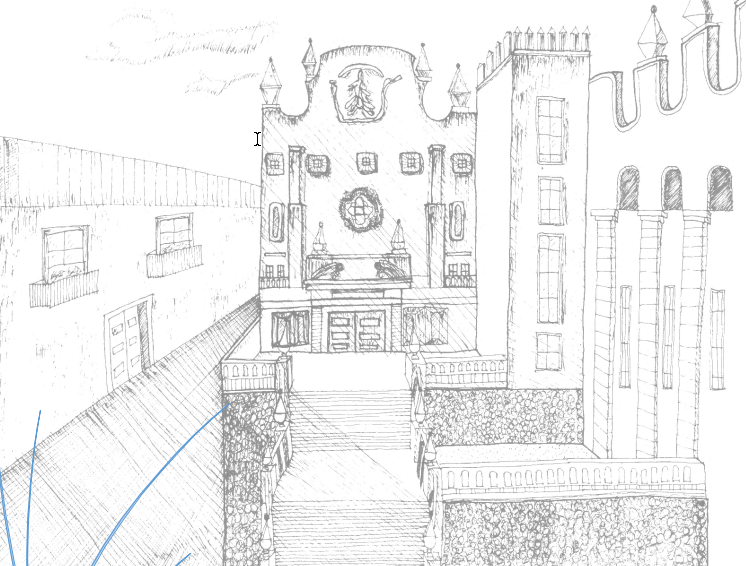
\includegraphics[width=18.0cm,height=9.5cm]{Imagenes/2}
		\vspace{1.6cm}
	    \end{center}
        %\begin{tcolorbox}[enhanced,frame style image=Imagenes/blueshade.png,opacityback=0.75,opacitybacktitle=0.25,colback=blue!5!white,colframe=blue!75!black,lifted shadow={1mm}{-2mm}{3mm}{0.1mm}{black!50!white}]
        %         	\hspace{4.5cm}  \textbf{Nombre: \hspace{0.2cm}Francisco Javier Mendoza Bautista \vspace{0.2cm} 
		%			\\ \hspace{4.5cm} Profesor: \hspace{0.1cm}Jose Luis López Ramírez \vspace{0.2cm}
		%			\\ \hspace{4.5cm} Tema: \hspace{0.7cm}Practica \#1 \vspace{0.2cm}
		%			\\ \hspace{4.5cm} Nua: \hspace{0.9cm}145645 \vspace{0.2cm}
		%			\\ \hspace{4.5cm} Email: \hspace{0.6cm}fj.mendozabautista}
        % \end{tcolorbox}
	    \begin{tcolorbox}
                 	\hspace{4.5cm}  \textbf{Nombre: \hspace{0.2cm}Francisco Javier Mendoza Bautista \vspace{0.2cm} 
					\\ \hspace{4.5cm} Profesor: \hspace{0.1cm}Jose Luis López Ramírez \vspace{0.2cm}
					\\ \hspace{4.5cm} Tema: \hspace{0.7cm}Practica \#1 \vspace{0.2cm}
					\\ \hspace{4.5cm} Nua: \hspace{0.9cm}145645 \vspace{0.2cm}
					\\ \hspace{4.5cm} Email: \hspace{0.6cm}fj.mendozabautista}     
        \end{tcolorbox}
	    \vfill 
        
		\begin{center}
         \today
		\end{center}
	    \end{titlepage}
     	\espacio{1}

		\sect{hola}
	    Crear una carpeta Imagenes para insertar desde la carpeta \\
        
		\section{Conclusiones}
		Ejemplo de conclusiones en formato IEEE
	%	\justify
         
		\begin{center}
			\begin{thebibliography}{1}
	
				 
				 \bibitem{B}Ogata Katsuhiko, “Sistemas de Control en Tiempo Discreto 2da Ed”, $2^{a}$ edición, Ed. Pearson, Madrid (España), 2010.
	
			\end{thebibliography}
			
		\end{center}    
		
		
		

		

	\end{document}

